\documentclass{beamer}


\usetheme{Warsaw}
\usecolortheme{crane}


\title{Groups \& Vector Spaces}
\subtitle{Mathematical Methods in the Physical Sciences}
\author{Steve Mazza}
\institute[Naval Postgraduate School]
{
  Naval Postgraduate School \\
  Monterey, CA \\
  
\includegraphics[height=3cm]{images/NPS_logo.jpg}
}
\date {SE3030, Winter/2014 \\ Quantitative Methods of Systems Engineering}
\subject{Quantitative Methods of Systems Engineering}


\begin{document}

\frame{\titlepage}


% \section{Groups}
\begin{frame}{Groups}
    \center{ 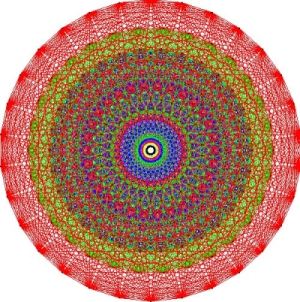
\includegraphics[height=0.7\textheight]{images/mandala.jpg} }
\end{frame}

\begin{frame}{Definition of Groups}
    A group is a set of elements, $G$, together with a set operation, $\cdot$, that satisfies the following conditions:
    \begin{block}{Group Conditions}
        \begin{description}
            \item [Closure: ] $\forall ~a, b \in G, a\cdot b \in G$
            \item [Association: ] $\forall ~a, b, c \in G, (a\cdot b)\cdot c = a\cdot(b\cdot c)$
            \item [Identity: ] $\exists$ exactly 1 element, $i \in G \mid \forall ~a \in G, i\cdot a = a\cdot i = a$
            \item [Inversion: ] $\forall ~a \in G ~\exists ~b \mid a\cdot b = b\cdot a = i$, where $i$ is the identity element.
        \end{description}
    \end{block}
\end{frame}

\begin{frame}{Operation Table}
    \begin{block}{Product}
        The term \emph{product} is used in the generalized sense.
    \end{block}
    It is handy to write out an operation table for the group.
    \begin{exampleblock}{Operation Table on $\pm 1, \pm i$}
        \begin{center}
            \begin{tabular}{c|cccc}
                & 1 & i & -1 & -i \\
                \hline
                1 & 1 & i & -1 & -i \\
                i & i & -1 & -i & 1 \\
                -1 & -1 & -i & 1 & i \\
                -i & -i & 1 & i & -1
            \end{tabular}
        \end{center}
    \end{exampleblock}
\end{frame}

\begin{frame}{Group Isomorphism}
    \begin{block}{Definition}
        $f: (G,\cdot)\rightarrow (H,\times) \mid \forall\ u, v \in\ G, f(u\cdot v) = f(u)\times f(v)$
    \end{block}
    Two groups are considered \emph{isomorphic} if an isomorphism exists between them.  We write $G\cong H$.  Isomorphic groups are considered indistinguishable.
\end{frame}

\begin{frame}{Group Symmetry}
    \begin{block}{Definition}
        The symmetry group is the group of all isometries under which the elements are invariant with regard to the group operation.
    \end{block}
    \center{ 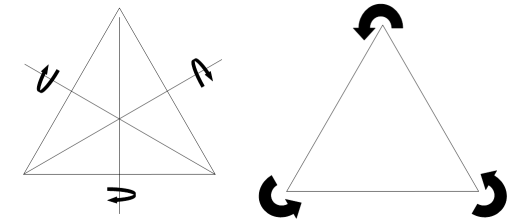
\includegraphics[height=0.25\textheight]{images/trianglesymmetries.png} }
    \begin{exampleblock}{Equilateral Triangle}
        We consider the example presented on Boas, page 174, where the equilateral triangle is symmetric on three reflections and three rotations.
    \end{exampleblock}
\end{frame}

\begin{frame}{Conjugate Elements, Class, Character}
    \begin{block}{Conjugate Elements}
        $a, b, \in\ G$ are called conjugate elements if $\exists\ c \in\ G \mid c^{-1}\cdot a\cdot c = b$.
    \end{block}
    All elements of a class describe the same mapping.
    \begin{block}{Class}
        The set of all elements conjugate to a given element form a \emph{class}.
    \end{block}
    Class is a subset of a group, but not a usually subgroup.  All matrices of a class have the same trace (sum of diagonal elements).
    \begin{block}{Character}
        The trace of a matrix is called its character.
    \end{block}
    All matrices of a class have the same character.
\end{frame}

\begin{frame}{Irreducible Representations}
    \begin{block}{Definition}
         If a group, $G$, only has two subrepresentations, $\emptyset$ and $G$, then $G$ is said to be irreducible.
     \end{block}
\end{frame}


% \section{Vector Spaces}
\begin{frame}{Vector Spaces}
    \center{ 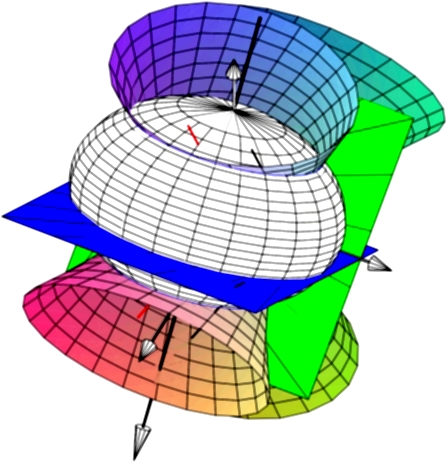
\includegraphics[height=0.7\textheight]{images/hyps-test.jpg} }
\end{frame}

\begin{frame}{Definition of Vector Spaces}
    A vector space over field $F$ is a set $V$ together with two binary operations satisfying following conditions:
    \begin{block}{Group Conditions}
        {\tiny
            \begin{description}
                \item [Closure: ] $\forall\ \vec{u}, \vec{v} \in V, \vec{u} + \vec{v} \in V$
                \item [Vector Addition:]\hfill
                \begin{description}
                    \item [Commutation: ] $\forall\ \vec{u}, \vec{v} \in V, \vec{u}+\vec{v}=\vec{v}+\vec{u}$
                    \item [Association: ] $\forall\ \vec{u}, \vec{v}, \vec{w} \in V, (\vec{u} + \vec{w}) + \vec{w} = \vec{u} + (\vec{v} + \vec{w})$
                \end{description}
                \item [Additive Identity: ] $\exists\ \vec{0} \in V \mid \forall\ \vec{v} \in V, \vec{0} + \vec{v} = \vec{v} + \vec{0} = \vec{v}$
                \item [Additive Inverse: ] $\forall\ \vec{v} \in V\ \exists\ -\vec{v} \mid \vec{v}+(-\vec{v}) =0$
                \item [Multiplication: ]\hfill
                \begin{description}
                    \item [Distribution 1: ] $\forall\ \vec{u}, \vec{v} \in V, k(\vec{u}+\vec{v}) = k\vec{u}+k\vec{v}$
                    \item [Distribution 2: ] $\forall\ \vec{v} \in V, \vec{v}(k_1+k_2)=k_1\vec{v}+k_2\vec{v}$
                    \item [Association: ] $\forall \vec{v} \in V, \vec{v}(k_1\cdot k_2)=(\vec{v}\cdot k_1)k_2$
                    \item [Identity: ] $\forall\ \vec{v} \in V, 1\cdot \vec{v}=\vec{v}$
                    \item [Zero: ] $\forall\ \vec{v} \in V, 0\cdot\vec{v} = \vec{0}$
                \end{description}
            \end{description}
        }
    \end{block}
\end{frame}

\begin{frame}{Inner Product, Norm, Orthogonality}
    For $A(x)$ and $B(x)$ on $a\leq x\leq b$, we define the following.
    \begin{block}{Inner Product}
        $\left <A(x), B(x) \right > = \int_a^b \overline{Ax}B(x)dx$
    \end{block}
    \begin{block}{Norm}
        $\lVert A(x)\rVert = \sqrt{\int_a^b \overline{Ax}A(x)dx}$
    \end{block}
    \begin{block}{Orthogonality}
        $A(x)\perp B(x)$ on $(a,b)$ if $\int_a^b \overline{Ax}B(x)dx=0$
    \end{block}
\end{frame}

\begin{frame}{Schwartz's Inequality}
    Let $\vec{u}, \vec{v}$ ab elements of a vector space.  Recall previously that for $n$-dimensional space, Schwartz's Inequality states
    \begin{block}{Schwartz's Inequality for $n$-dimensional Space}
        $\lvert\vec{u}\cdot\vec{v}\rvert\leq AB$
    \end{block}
    For an inner product space, we modify the definition as follows.
    \begin{block}{Schwartz's Inequality for Inner Product Space}
        $\lvert\left<\vec{u}\mid\vec{v}\right>\rvert^2\leq\left<\vec{u}\mid\vec{u}\right>\left<\vec{v}\mid\vec{v}\right>$
    \end{block}
    Boas develops a proof of this on page 182.
\end{frame}

\begin{frame}{Orthonormal Basis}
    Two functions are \emph{orthonormal} if they
    \begin{itemize}
        \item satisfy the property of orthogonality, and
        \item have a norm $= 1$
    \end{itemize}
\end{frame}

\begin{frame}{Infinite Dimensional Spaces}
    An \emph{infinite dimensional vector space} is one which does not have a finite basis.
    \par We recall that the set of all linearly independent vectors $\vec{b_i}$ which, expressed as some finite sum, are capable of describing any vector, $\vec{v}$, form the \emph{basis} for our vector space.
    \par As an example, consider $\mathbb{R}[x]$, the set of polynomials in $x$ with real coefficients for which ${x:n\in\mathbb{N}}$ forms the basis.
\end{frame}

\begin{frame}{Questions?}
	\begin{center}
		
\includegraphics[width=.7\textwidth]{images/fin.png}
	\end{center}
\end{frame}

\end{document}
